	%% The following is a directive for TeXShop to indicate the main file
%%!TEX root = diss.tex

\chapter{Introduction}
\label{ch:Introduction}

\begin{epigraph}
    \emph{If I have seen farther it is by standing on the shoulders of
    Giants.} ---~Sir Isaac Newton (1855)
\end{epigraph}

Computational Fluid Simulations (CFD) is a field of study where scientists and engineers architect new ways to numerically solve fluid flow equations. Before the advent of computers, numerical solutions of differential equations was done by hand. This lead to a great deal of work in the direction of creating faster algorithms to solve differential equations. An example is the development of the Fast Fourier Transform (FFT) by Cornelius Lancoz to increase the computation speed of Discrete Fourier Transform (DFT). However, since the development and advancement of computers, engineers had a significant amount of compute power to work with. This lead to the development of highly accurate methods (as compared to before) to simulate flow over various objects. These simulations have since gotten bigger and better, typically including millions of degrees of freedom, even starting to touch a billion in regular industry use.

\subsection{Mesh Generation - A brief overview}

The equations which govern the conservation of mass, momentum and energy of a moving fluid also called Navier-Stokes equations are solved in the given domain to simulate fluid flow in that domain. In order to numerically solve these equations, we need a discretization of the given domain. This discrete basis required to solve the Navier-Stokes equations is called a mesh. Simply put, a mesh is a collection of points, lines and cells that together construct the space around a body in a fluid flow.

The process of discretization of the domain to form the basis of solving the Navier-Stokes equations, or any other differential equation numerically is called mesh generation. Save a few exotic methods, almost all of the techniques in CFD require a mesh to solve the flow on. Traditionally, mesh generation was a very manual process, where engineers used to place the mesh points and cells by hand. Such heuristic approach to mesh generation gave them a lot of freedom in discretizing the domain. Cells could be aligned to the boundaries of objects. The quality of the cells, which was taken as some measure of the interior angle of the cells, was almost always chosen to be good. The benefits of this method were quite evident. However, there were some major drawbacks. The process of mesh generation was incredibly slow. Engineers would spend hours, sometime days to create the mesh for a given geometry. Also, mesh adaptation with solution was almost non-existant because that would have made the process even slower.

\begin{definition}
A mesh $M$ is a geometrical discretization of a domain $\Omega$ that consists of (a) a collection of mesh entities $M_i$ of controlled size and distribution and (b) topological relationships or adjacencies forming the graph of the mesh. The mesh $M$ covers $\Omega$ without neither overlap nor hole.
\end{definition}

\begin{figure}
  \centering
  \begin{subfigure}{0.5\linewidth}
    \centering
    \includegraphics[width=0.8\linewidth]{img/intro/mStructured.png}
    \caption{}
    \label{fig-structured-ij}
  \end{subfigure}%
  \begin{subfigure}{0.5\linewidth}
    \centering
    \includegraphics[width=0.8\linewidth]{img/intro/mUnstructured.png}
    \caption{fig-unstructured-ij}
    \label{fig-unstructured}
  \end{subfigure}%
  \caption{}
  \label{fig-structured-unstructured}
\end{figure}

\subsection{Structured and Unstructured Meshes}

The evolution of mesh generation can be correlated to the evolution of compute power available to the boffins. With the advent of third generation computers (1964-1971) carryinig integrated circuits, engineers were able to automate some of the manual processes in mesh generation. Meshes consisting of a template that repeats itself could be generated. These meshes were called \textit{structured meshes} as their adjacencies or relationships could be known implicitly. Consider a grid in two dimensions as shown in Figure \ref{fig-structured-ij}. Given a cell $(i,j)$ we can identify its neighbours as $(i-1, j)$ to the left and $(i+1, j)$ to the right. Similarly, cell $(i, j+1)$ will be to the top and $(i, j-1)$ would be to its bottom. The connectivity pattern repeats in such a mesh. Figure \ref{fig-structuredNaca0012} shows a structured mesh generated for NACA 0012 airfoil around its leading edge. Notice the implicit connectivity of the cells even though the size of mesh elements is varying.

\begin{figure}
  \centering
  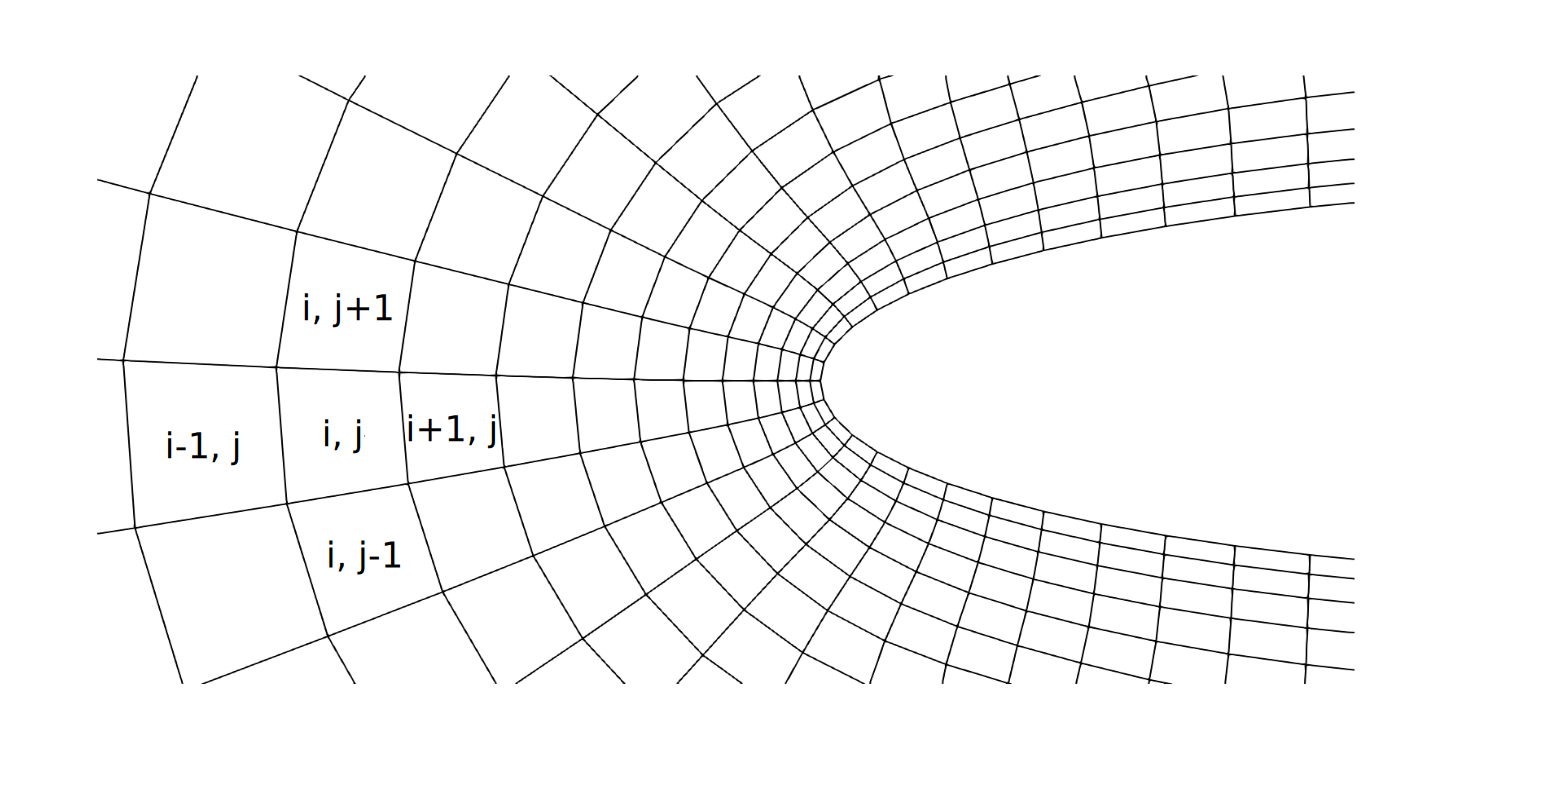
\includegraphics[width=0.6\linewidth]{img/intro/stucturedNaca0012.png}
  \caption{Structured mesh around leading edge of a NACA 0012 airfoil}
  \label{fig-structuredNaca0012}
\end{figure}


Structured meshes were attractive to engineers because of their low memory usage as the topology of the cells is repeated. Also, given simple domains to mesh, these meshes were optimal for minimizing the errors in CFD, resulting in faster simulations \cite{d1991optimal}. Programming CFD solvers with these meshes was easy as cell connectivity occurs in a regular fashion. However, as the scope of CFD simulations grew over time and more complex geometries were becoming commonplace, the task of generating structured meshes around them proved to be a daunting one. 

The disadvantage of using a structured mesh for more complex geometries is the increase in grid non-orthogonality or skewness that can cause unphysical solutions due to the transformation of the governing equations\cite{TU2013219}. The transformed equations that accommodate the non-orthogonality act as the link between the structured coordinate system (such as Cartesian coordinates) and the body-fitted coordinate system, but contain additional terms, thereby augmenting the cost of numerical calculations and difficulties in programming. Hence, a structured mesh may affect the accuracy and the efficiency of the numerical schemes used by a solver. Additionally, the tedious process of generating such meshes for more complex geometries was hard to justify. Hence, more flexible and automatic methods were devised. These methods produced meshes in a more random manner but with lesser human intervention. Broadly, the meshes produced by such methods were classified as \textit{unstructured meshes}. Figure \ref{fig-unstructured} shows an unstructured mesh. The arrangement of the mesh elements is random. Along with the shape of the elements, we need a data structure to store the adjacencies of the mesh.

The cost of finding flux at a wall, a widely used parameter in Finite Volume Methods (FVM), for unstructured meshes is high as compared to their structured counterparts. Also, the amount of memory usage is also high as the topology of the mesh is no longer repeated. Still, they are more widely used today because of their capability to handle arbitrary complex geometries, their capability to automate the mesh generation process and their flexibility in refinement based on the geometry topology and/or the solution gradients. Figure \ref{fig-unstructuredNaca0012} shows an unstructured mesh at the leading edge of a NACA 0012 airfoil. Notice the random arrangement of triangles around the airfoil geometry. The connectivity at each vertex of the mesh needs to be stored separately.

\begin{figure}
  \centering
  \includegraphics[width=0.6\linewidth]{img/intro/unstructuredNaca0012.png}
  \caption{Unstructured mesh around leading edge of NACA 0012 airfoil}
  \label{fig-unstructuredNaca0012}
\end{figure}

\section{Boundary Layer Meshes}

With the advent of several unstructured mesh generation techniques (cite them), a broader selection of geometries could be dealt with. This immensely increased the scope of CFD solvers and pushed the limits of numerical methods in terms of accuracy and speed. However, a different approach was needed for the parts of the mesh in which viscous forces were more dominant as compared to the inertial forces. In other words, at the location of the viscous boundary layer, a mesh generation technique which would help in resolving the strong gradients of the velocity in the direction normal to the boundary was required. For example, consider a flow over an airfoil. The velocity of the fluid at the surface of the airfoil is zero. However, the velocity becomes freestream velocity very near to the surface. The thickness of this layer of fluid, where the freestream velocity goes from a value of zero to a value of around 0.95 times the freestream velocity is called as the boundary layer. It is also called the viscous boundary layer as the viscous effects are dominant in this layer.

\section{Anisotropic Meshing}

\section{Objective and Outline}
